\documentclass[10pt]{beamer}
\usepackage[english, russian]{babel}
\usepackage{setspace, amsmath}
\usepackage{color}
\usepackage{multicol}
\usetheme{Pittsburgh}
\begin{document}
	\defbeamertemplate*{frametitle}{shadow theme}{
		\vskip 2pt \leavevmode
		\hbox to \paperwidth {
			\hbox to 2.5cm {
				\hskip -28pt \vbox to -2pt {
					\vskip-14pt 
\includegraphics[width=2.5cm] {logo.png}
				}
			}
			\begin{beamercolorbox}[wd=\paperwidth,ht=2ex,dp=3pt,left]{title in head/foot}
				\insertframetitle
			\end{beamercolorbox}
		}
	}
	
  
	\begin{frame}
		 \frametitle {{\color{blue}А}нализ свойств меры Хартли}
		Экспериментатор одновременно подбрасывает монету (М) и кидает игральную кость (К).\\
		Какое количество информации содержится в эксперименте (Э)?
		\vskip 0.5cm
		\textbf{Аддитивность}:\\
		\quad $i($Э$) = i($М$) + i($К$) \Rightarrow i(12 исходов) = i(2 исхода) + i(6 исходов): \log_x 12 = \log_x 2 + \log_x 6$\\
		\vskip 0.3cm
		\textbf{Неотрицательность}:\\
		\quad Функция $\log_x N$ неотрицательно при любом $x > 1$ и $N \geq 1$.\\
		\vskip 0.3cm
		\textbf{Монотонность}:\\
		\quad С увеличением $p($М$)$ или $p($К$)$ функция $i($Э$)$ монотонно возрастает.\\
		\vskip 0.3cm
		\textbf{Принцип предопределённости}:\\
		\quad При наличии всегда только одного исхода (монета и кость с 
		\phantom \quad магнитом) количество  информации равно нулю: $\log_x 1 + \log_x 1 = 0$.\\
    	\end{frame}
	\begin{frame}
	\begin{minipage}[b]{0.70\textwidth}
		\frametitle {{\color{blue}М}ера количества информации по Шеннону}
		\small Мера Хартли подходит лишь для систем м равновероятными состояниями. \\
		Если состояния системы S не равновероятны, используют меру Шеннона:
	\begin{center}
		\textit{i(S) = $\sum$ $p_i$*$\log_2$$p_i$},
	\end{center}
		\normalsize где \textit{N} -- число состояний системы,\\
		\textit{$p_i$} -- вероятность того, что система S находится в\\
		\quad состоянии \textit{i} (сумма всех \textit{$p_i$} равна 1).
	\end{minipage}
	\begin{minipage}[b]{0.20\textwidth}
		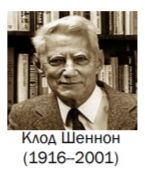
\includegraphics[width=3cm,height=3cm]{present_2.png}\\
	\end{minipage}
	\begin{center}
		{\color{green}Формула Хартли является частным случаем формулы Шеннона!}
	\end{center}

		\small \textbf{Пример 1.} Количество информации в акте подбрасывания обычной\\
		 монеты по формуле Хартли равно $\log_2$2 = 1 бит. По формуле Шеннона\\
		получим то же:${i_s}_1 = -0,5*\log_2 0,5 - 0,5*\log_2$ 0,5 = 1 бит.\\
		\textbf{Пример 2.} При подбрасывании монеты со смещенным центром тяжести\\
		 количество непредсказуемости становится меньше:${i_s}_2 = -0,75*\log_2 0,75 - 0,25*\log_2 0,25 \approx$ 0,8 бит.
		
	\end{frame}

	\begin{frame}
		\frametitle {{\color{blue}П}ример использования меры Шеннона}
		Шулер наугад вытаскивает одну карту из стопки, содержащей 9 \\
		известных ему карт: 3 джокера, 3 туза, 1 король, 1 дама и 1 валет.\\
		Какое количество информации для шулера содержится в этом событии s?
	\begin{equation*}
		\text{Вероятность вытащить} = 
 		\begin{cases}
 			$джокера$\\
   			$туза$\\
			$короля$ \\
			$даму$\\
			$валета$
		 \end{cases}
		\text{равна}
		\begin{cases}
			3/9 = 1/3\\
			3/9 = 1/3\\
			1/9\\
			1/9\\
			1/9
		\end{cases}
	\end{equation*}

		Количество информации, выраженное в тритах, равно:\\
		
		\textit{i(s)} = -($\frac{1}{3}$*$\log_3$ $\frac{1}{3}$ + $\frac{1}{3}$ * $\log_3$  $\frac{1}{3}$ +  $\frac{1}{9}$ * $\log_3$  $\frac{1}{9}$ +  				$\frac{1}{9}$*$\log_3$ $\frac{1}{9}$ + $\frac{1}{9}$*$\log_3$ $\frac{1}{9}$ = \\
	\begin{center}
		= $\frac{1}{3}$ + $\frac{1}{3}$ + $\frac{2}{9}$ + $ \frac{2}{9}$ + $ \frac{2}{9}$ = 1$\frac{1}{3}$ $\approx$ $\log_3$5 vs $\log_3$14
	\end{center}
	\end{frame}

	\begin{frame}
		\frametitle {{\color{blue}Н}естрогий вывод формулы Шеннона}
		{\color{green}Задача}. Монета имеет смещенный центр тяжести. Вероятность \\
		выпадения <<орла>> -- 0,25, вероятность выпадения <<решки>> -- 0,75. \\
		Какое количество информации содержится в одном подбрасывании?\\
		\vspace{0.5cm}
		{\color{green}Решение}\\
		\small $\bullet$ \quad Пусть монета была подброшена \textit{N}  раз (\textit{N}$\implies$ $\infty$  ) из которых\\
		 \qquad <<решка>> выпала \textit{M} раз, <<орел>> --\textit{K} раз (очевидно, что \textit{N = M + K}).\\

		$\bullet$ \quad Количество информации и в N подбрасываниях: \textit{$i_N$ = M*i( <<решка>>)\\
		\qquad + K*i(<<орел>>)}.

		$\bullet$\quad Тогда среднее количество информации в одном подбрасывании:\\
		\qquad $i_1$ = $i_N$/ = (M/N)*i(<<решка>>)+(K/N)*i( <<орел>>) = p(<<решка>>)*\\
		\qquad *i(<<решка>>)+p( <<орел>>)*i( <<орел>>).

		$\bullet$ \quad Подставив формулу Шеннона для \textit{i}, оконачательно получим:\\
		\qquad $i_1$ = -p(<<решка>>)*$\log_xp$(<<решка>>) - p(<<орел>>)*$\log_xp$(<<орел>>) $\approx$ 0,8\\
		\qquad бит.
	\end{frame}
	\begin{frame}
		\frametitle {{\small \color{blue} П}\small риставки для единиц измерения количества информации/данных}
		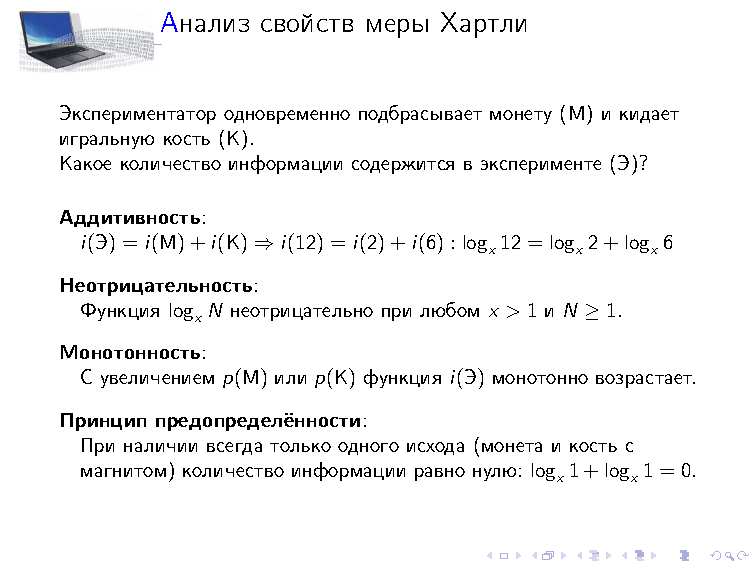
\includegraphics[width=11cm, height=5cm]{present_1.png}\\
	\begin{center}
		\textbf{ 33 097 216 байт -- это {\color{green}33,1} МБ или {\color{green}31,5} МБ?}
	\end{center}

	\end{frame}
\end{document}

